% Roll Number 17, Arjun K

\textbf{\textcolor{LightMagenta}{Consider the training data in the following table where Play is a class attribute. In the table, the Humidity attribute has values “L” (for low) or “H” (for high), Sunny has values “Y” (for yes) or “N” (for no), Wind has values “S” (for strong) or “W” (for weak), and Play has values “Yes” or “No”.
\begin{figure}[htp]
    \centering
    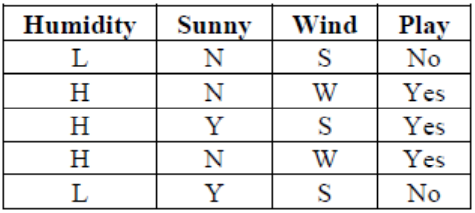
\includegraphics[width=10cm]{Images/A11_img1.png}
\end{figure}\\
What is class label for the following day (Humidity=L, Sunny=N,
Wind=W), according to naive Bayesian classification? (September 2020 - Q15b) \hfill 4 marks}} \\[5pt]

We have given a table of instances and the corresponding target values for play class attribute.\\
We have to classify new instance {Humidity=L, Sunny=N, Wind=W} and find the target value, whether its YES or NO.\\
P(play = yes)= 3/5 = 0.6\\
P(play = no) = 2/5 = 0.4\\
\begin{figure}[htp]
    \centering
    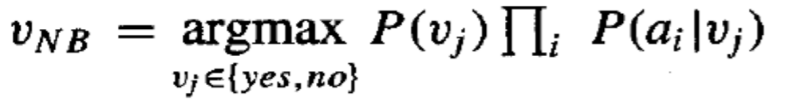
\includegraphics[width=10cm]{Images/A11_img2.png}
\end{figure}\\
So for calculating the probability for the given instances,\\
\textbf{P(v)P(humidity=low/v)P(sunny=no/v)P(wind=weak/v)}, where v $\epsilon$ {yes/no}.\\
P(yes)P(humidity=low/yes)P(sunny=no/yes)P(wind=weak/yes)\\
P(no)P(humidity=low/no)P(sunny=no/no)P(wind=weak/no)\\
P(humidity=low/yes) = 0/3 = 0\\
Here a condition occurs, model will assign a 0 (zero) probability and will be unable to make a prediction. It is called Zero frequency. To solve this issue, we can use smoothing technique. So we have to add smoothing parameter $\alpha=1$ and k=2(number of values in class).\\
P(humidity=low/yes) = 0+1/3+2 = 1/5 = 0.2\\
P(sunny=no/yes) = 2/3 = 0.67\\
P(wind=weak/yes) = 2/3 = 0.67\\
P(yes) = 0.6\\
P(yes)P(humidity=low/yes)P(sunny=no/yes)P(wind=weak/yes) = 0.6*0.2*0.67*0.67 = 0.054\\\\
P(humidity=low/no) = 2/2 = 1\\
P(sunny=no/no) = 1/2 = 0.5\\
P(wind=weak/no) = 0+1/2+2 = 1/4 = 0.25\\
P(no) = 0.4\\
P(no)P(humidity=low/no)P(sunny=no/no)P(wind=weak/no) = 0.4*1*0.5*0.25 = 0.05\\\\
Since probability of play=yes is 0.054 and play=no is 0.05, we know that its sum should be equals 1. For this we have to done normalization.\\
P(play=yes) = 0.054/(0.054+0.05) = 0.52\\
P(play=no) = 0.05/(0.054+0.05) = 0.48\\
Since P(play=yes)+P(play=no) = 0.52+0.48 = 1\\
We can assume that according to naive Bayesian classification class label for the following day with attributes(Humidity = L, Sunny = N, Wind = W) is yes.\\
